\documentclass[10pt,a4paper]{article}
\usepackage[utf8]{inputenc}\usepackage{pdfsync}
\usepackage[T1]{fontenc}
\usepackage{amsmath}
\usepackage{amsfonts}
\usepackage{amssymb}
\usepackage{amsthm}
\usepackage{xcolor}
\usepackage{bbm,graphicx}
\usepackage[left=2cm,right=2cm,top=2cm,bottom=2.5cm]{geometry}
\usepackage{subcaption}
\usepackage{hyperref}
\baselineskip=14.4pt \topmargin=-0.2cm\textwidth=16.45cm %\textheight=658pt
\textheight=23cm
\oddsidemargin=-0.65cm\evensidemargin=-0.65cm\headsep=20pt

\newtheorem{thm}{THEOREM}%[section]
\newtheorem{assumption}[thm]{ASSUMPTION}
\newtheorem{cor}[thm]{COROLLARY}
\newtheorem{lem}[thm]{Lemma}
\newtheorem{definition}[thm]{DEFINITION}
\newtheorem{example}[thm]{EXAMPLE}
\newtheorem{proposition}[thm]{PROPOSITION}
\newtheorem{remark}[thm]{REMARK}
\def\beXa{\begin{example}} \def\eeXa{\end{example}}
\def\eeD{\end{definition}} \def\beD{\begin{definition}}
\def\beR{\begin{remark}} \def\eeR{\end{remark}}
\def\beL{\begin{lem}} \def\eeL{\end{lem}}
\def\beP{\begin{proposition}} \def\eeP{\end{proposition}}
\def\beC{\begin{cor}} \def\beT{\begin{thm}}
  \def\eeT{\end{thm}}
\def\eeC{\end{cor}}
\def\intr{introduction } \def\lc{loading coefficient}
\def\Ic{In conclusion, }\def\Nat{Note also that }
\providecommand{\norm}[1]{\left\lVert#1\right\rVert}%//.//
\providecommand{\abs}[1]{\left\lvert#1\right\rvert}
\providecommand{\pr}[1]{\left(#1\right)} %(.)
\providecommand{\pp}[1]{\left[#1\right]} %[.]
\providecommand{\set}[1]{\left\lbrace#1\right\rbrace} %{.}
\providecommand{\scal}[1]{\left\langle#1\right\rangle}%<.>

%local commands
\providecommand{\Ptwo}{\mathcal{P}_2\pr{\mathbb{R}^d}}
\providecommand{\Ltwo}[1]{\mathbb{L}_{\mathcal{F}_{#1}}^2\pr{\mathbb{R}^d}}

\providecommand{\keywords}[1]{\textbf{\textit{Keywords:  }} #1}
\providecommand{\classification}[1]{\textbf{\textit{MSC:  }} #1}
%\providecommand{\EF}[1,2]{\mathbb{E}^{\mathcal{F}_{#1}}\pp{#2}}

\providecommand\eqD{\stackrel{\mathcal{D}}{=}}

\newcommand{\ex}{\mathbb{E}} \def\ssec{\subsection} \def\Kol{Kolmogorov }
\def\equ{equation } \def\BC{boundary condition } \def\fund{fundamental } \def\boun{boundary } \def\con{condition } \def\rv{random variable } \def\ind{independent } \def\opt{optimization }
\def\pb{problem }  \def\pbs{problems } \def\appr{approximation}
 \def\iid{i.i.d. } \def\adj{adjustment coefficient } \def\Tc{\tilde{c}} \def\Tq{\tilde{q}} \def\Tl{{\tilde{\lambda}}}  \def\mW{{\mathcal W}} \def\w{{\mathbf w}}  \def\fun{function } \def\funs{functions } \def\rui{\psi}
\def\GS{Gerber-Shiu } \def\vars{random variables }\newcommand{\bff}[1]{{\mbox{\boldmath$#1$}}}
\def\ts{two-sided } \def\wk{well-known } \def\pros{probabilities }
\def\prop{proportionality } \def\ct{constant } \def\cts{constants } \def\para{parameter} \def\paras{parameters} \def\wr{with respect to }
 \def\sub{subordinator } \def\rps{ruin probabilities} \def\ren{renewal equation } \def\JJ{Jacobsen }
\newcommand{\df}{\mathrm{d}} \def\wk{well-known} \def\ts{two sided exit }
\newcommand{\dint}{\displaystyle\int}
\def\G{\Gamma}
 \def\bs{\bigskip } \def\res{respectively}
\newcommand{\kil}{\mathbf{e}} \def\procs{processes} \def\proc{process}
\def\Rui{\Psi} \def\sRui{\ovl{\Rui}}
\newcommand{\di}{{\rm d}} \def\fp{first passage }
\def\ovl{\overline}\def\tzp{T_{0,+}}
\def\lev{L\'evy }  \def\mL{{\mathcal L}} \def\rp{ruin probability} \def\expc{exponential claims}\def\Oth{On the other hand, }
\def\dd{draw-down } \def\sn{spectrally negative }
\long\def\symbolfootnote[#1]#2{
\begingroup
\def\thefootnote{\fnsymbol{footnote}}\footnote[#1]{#2}
\endgroup}
\def\fn{\symbolfootnote}
\def\den{denominator }
\def\I{\infty} \def\Eq{\Leftrightarrow}
\def\und{\underline} \def\unl{\underline} \def\T{\widetilde}
\def\CL{Cram\'er-Lundberg } \def\WH{Wiener-Hopf } \def\iof{l^{-1}(a)}
\def\SA{Sparre-Andersen } \def\PH{phase-type }  \def\sat{satisfy }
\def\BEN{\begin{enumerate}}  \def\BI{\begin{itemize}}
\def\EEN{\end{enumerate}}   \def\EI{\end{itemize}} \def\im{\item} \def\Lra{\Longrightarrow} \def\De{\Delta} \def\eqr{\eqref} \def\mpr{more precisely, } \def\cof{coefficient}
\def\no{\nonumber} %\newcommand{\be}{\begin{equation}}
%\newcommand{\ee}{\end{equation}}
\def\mG{{\mathcal G}}
\def\g{\gamma}  \def\d{\delta} \def\de{\delta}  \def\b{\beta}
\def\z{\zeta}  \def\th{\theta} \def\vt{\vartheta}
\def\e{\epsilon} \newcommand{\ol}{\overline}
\def\k{\kappa} \def\l{\lambda} \def\a{\alpha} %\def\W{W}
\def\Lm{L\'evy measure } \def\thf{therefore } \def\mgf{moment generating function } \def\resp{respectively} \def\how{however} \def\SLG{Shreve, Lehoczky and Gaver} \def\snp{spectrally negative \lev \procs} \def\PK{Pollaczek-Khinchine } \def\LZ{Lokka-Zervos alternative}
\def\lm{\Pi} \def\x{\xi} \def\ith{it holds that } \def\sf{scale function}
  \def\r{r} \def\Sp{\Seg \proc}\def\s{\sigma} \def\F{\Phi} \def\Fql{\Phi_{\q+\l}}\def\fmi{for more information}
  \def\Fq{\Phi_{\q}}\def\f{\varphi}\def\L{L} \def\U{D}
  \def\satd{satisfied} \def\Z1{Z_{\q,1}}
  \def\bc{\begin{cases}
  } \def\gene{generalization }  \def\levs{\lev processes } \def\wlg{w.l.o.g. } \def\cP{compound Poison model }
\def\ec{\end{cases}} \def\expo{exponential } \def\CIR{Cox-Ingersoll-Ross }
  \def\qu{\quad} \def\for{\forall}
  \def\beq{\begin{eqnarray}} \def\eeq{\end{eqnarray}}
   \def\be{\begin{equation}} \def\ee{\end{equation}}
\def\bea{\begin{eqnarray*}} \def\rei{reinsurance } \def\adj{adjustment coefficient }\def\mbw{may be written as }\def\Equ{Equivalently, }\def\ms{must satisfy }
  \def\prf{{\bf Proof:} } \def\satg{satisfying } \def\Eb{\E^{b]}}
\def\eea{\end{eqnarray*}} \def\la{\label}
\def\LE{Laplace exponent } \def\LT{Laplace transform} \def\BM{Brownian motion}\def\perf{performance}
\def\LTs{Laplace transforms} \def\q{q} \def\R{{\mathbb R}}
\def\le{\left} \def\ri{\right}
\def\nne{nonnegative } \def\fr{\frac} \def\Y{Y}  \def\t{\tau} \def\ta{T_{a,-}}  \def\tb{T_{b,+}}  \def\tret{T_{\{0\}}}
\def\tz{T_{0,-}} \def\sec{\section} \def \fe{for example } \def\wlo{w.l.o.g. }  \def\ith{it holds that }\def\genr{generator}
\def\itf{it follows that } \def\sev{severity of ruin}
\newcommand{\goto}{\rightarrow} \def\deF{de Finetti } \def\app{approximation}
\def\oedd{optimal expected discounted cumulative dividends }
\def\edd{expected discounted cumulative dividends }
%\theoremstyle{definition}
 \def\A{\mathcal A} \def\valf{value function}
\newcommand{\bE}{\mathbb{E}} \def\bsq{\qed} \def\sur{survival }
\def\Ip{In particular, } \def\cP{compound Poisson }
\def\pros{probabilities } \def\fund{fundamental }
\def\rvs{random variables } \def\rv{random variable } \def\gen{generalized }
\def\nonh{nonhomogeneous } \def\Frt{Furthermore, } \def\expo{exponential } \def\pro{probability }
\def\prob{problem} \def\probs{problems }  \def\ts{two-sided exit }
\def\how{however } \def\How{However, } \def\H{\widehat }
\def\mC{\mathcal C}  \def\os{one-sided } \def\Ga{\Gamma}
\def\1{\mathop{\rm 1\!\!I}\nolimits}   \def\HG{\widehat{G}}
\def\mH{\mathcal H} \def\mZ{{\mathcal Z}}  \def\mW{{\mathcal W}}
\newcommand{\pd}[2]{\frac{\partial #1}{\partial #2}}
\newcommand{\pdn}[3]{\frac{\partial^{#3} #1}{\partial #2^{#3}}} \def\Seg{Segerdahl } \def\rf{retention function }\def\drp{dynamic reinsurance policy }
\def\prob{problem} \def\probs{problems} \def\proba{probability} \def\str{strong Markov property}
\def\frt{furthermore } \def\nonh{nonhomogeneous } \def\td{\tau} \def\probas{probabilities} \def\ma{master equation } \def\ker{\varphi_{0}} \def\brp{branching point} \def\dz{\; \fr {d z}{z}}
\def\strs{strong Markov processes} \def\vfe{}  \def\Ez{\E^{[0}} \def\AY{Azema-Yor } \def\KWP{Kolmogorov-Wong-Pearson }
\def\splp{spectrally positive L\'evy process}
\def\cci{complex contour integrals} \def\mcci{the method of complex contour integrals} \def\cgf{cumulants generating function }
  \def\Itf{It follows that } \def\Mcci{The method of complex contour integrals } \def\wh{where } \def\Ea{\E^{[a}} \def\Eb{\E^{b]}}
\newcommand{\E}{{\rm I \!E}} \def\OU{Ornstein-Uhlenbeck } \def\difs{diffusions} \def\mex{mixed exponential jumps }
\newcommand{\p}{{\rm I \!P}} \def\sp{spectrally positive } \def\dif{diffusion}
 \newcommand{\md}{\mathrm d}  \def\mI{\mathcal I} \def\divs{dividends }
\newcommand{\red}{\textcolor[rgb]{1.00,0.00,0.00}}
\newcommand{\blue}{\textcolor[rgb]{0.00,0.00,1.00}}
\newcommand{\green}{\textcolor[rgb]{0.00,1.00,0.00}}
\newcommand{\W}[2]{\ensuremath{W^{(#1)}(#2)}}
\newcommand{\dW}[2]{\ensuremath{W^{(#1)\prime}(#2)}}
%\newcommand{\Z}[2]{\ensuremath{Z^{(#1)}(#2)}}
%\newcommand{\dZ}[2]{\ensuremath{Z^{(#1)\prime}(#2)}}
\newcommand{\ddZ}[2]{\ensuremath{Z^{(#1)\prime\prime}(#2)}}
\def\TV{\tilde{V}_q(0)} \def\Beta{\mathfrak B}
\def\Ezz{\E^{[0[}} \def\Ezb{\E^{[0,b]}} \def\Pzb{P^{[0,b]}}
   \def\Eazr{\E^{|0,b[}} \def\Eazb{\E^{|0,b]}} \def\sd{scale derivative }
   \def\Vb{V^{b]}} \def\Vkb{V_k^{b}} \def\Vr{V^{b[}} \def\Vzr{V^{[0,b[}}
   \def\Vzz{V^{[0[}} \def\Vzb{V^{[0,b]}} \def\Thr{Therefore, }
   \def\Fr{Furthermore, } \def\frt{furthermore } \def\app{approximation}\def\woF{\widehat{\overline{\lm}}}
   \def\Vazr{V^{|0,b[}} \def\iffa{} \def\Xt{(X_t)_{t \geq 0}} \def\mZ{{\mathcal Z}} \def\mA{\mathcal A} \def\mB{\mathcal B} \def\mC{\mathcal C} \def\mU{\mathcal U} \def\mI{\mathcal I} \def\ubd{unbounded variation case} \def\mR{\mathcal R}
\def\bd{bounded variation case} \def\div{dividend} \def\rd{reserves-dependent } \def\val{value function}\def\Pd{Pad\'e approximation } \def\Pds{Pad\'e approximations}\def\tPd{two point Pad\'e approximation} \def\pcs{particular cases of } \def\pc{particular case of }
   \def\cmy{complete monotonicity } \def\Lm{L\'evy measure }\newcommand{\eps}{\varepsilon} \def\wkt{well-known and easy to check that } \def\expoc{exponential claims}
   \def\Mp{More precisely, } \def\sats{satisfies} \def\form{formula } \def\sat{satisfy} \def\fun{function } \def\expl{explicit } \def\funs{functions} \def\thr{therefore } \def\wf{we find that } \def\inc{increasing} \def\resp{respectively} \def\proc{process} \def\eq{equation} \def\eqs{equations} \def\cd{(\cdot)} \def\sat{satisfy} \def\ci{capital injections} \def\C{C} \def\D{D} \def\tRui{| \Rui} \def\uph{\red{UP TO HERE}}
\def\abs{absolute } \def\part{\partial } \def\tx{T_{x,+}}  \def\te{T_{\e,+}} \def\iLT{inverse Laplace transform  }\def\bep{\begin{pmatrix}} \def\eep{\end{pmatrix}}
   \def\ito{it turns out that } \def\bcons{boundary conditions} \def\bcon{boundary condition } \def\SL{Sturm Liouville } \def\wrt{with respect to }\def\rmi{\rho_{-}} \def\rpl{\rho_{+}}
   \def\nny{nonnegativity } \def\wth{with respect to } \def\abr{absolute ruin } \def\PHj{phase-type jumps} \def\tZ{\;{^| Z}} \def\tW{\;{^| W}} \def\tRui{\;{^| \Rui}} \def\inth{in the case of } \def\c{c} \def\ctr{control } \def\eddc{expected discounted dividends minus capital injections}\def\coe{coefficient} \def\per{perturbed } \def\Ito{It turns out that }\def\std{state dependent } \def\Marp{Markov process} \def\saty{satisfy } \def\wft{we find that }\def\LTW{Laguerre-Tricomi-Weeks}\def\TW{W^{(\Fq)}_0} \def\FT{fixed Talbot algorithm }\def\ET{Esscher transform}\def\WF{W^{(\Fq)}}
   \def\ratap{rational approximation}
   \def\Dis{\mathfrak D} \def\Mar{Markov }\def\fac{factorization} \def\DW{\Delta^{(W)}_\q} \def\DZ{\Delta^{(Z)}_\q} \def\CLp{\CL process  } \def\form{formula} \def\fno{from now on} \def\upc{up to a constant} \def\snl{\sn \lev \procs } \def\expoj{exponential jumps} \def\prc{proportionality constant} \def\Itt{It turns out that }\def\snL{spectrally negative L\'evy processes} \def\wr{with respect to }\def\Tse{This is equivalent to }\def\LZa{Lokka-Zervos alternative}\def\GSf{\GS function}\def\sta{standard }\def\deV{de Vylder approximation}\def\wmh{we must have }\def\Ite{It is enough to analyze }
   \def\Tse{This is equivalent to }\def\elts{elements }\def\capi{capital injections}\def\edd{expected discounted dividends }\def\obj{objective} \def\ti{\times } \def\tc{T_{c,+}} \def\tbm{T_{b,-}}\def\Nt{Note that }
\providecommand{\norm}[1]{\left\lVert#1\right\rVert}%//.//
\providecommand{\abs}[1]{\left\lvert#1\right\rvert}
\providecommand{\pr}[1]{\left(#1\right)} %(.)
\providecommand{\pp}[1]{\left[#1\right]} %[.]
\providecommand{\set}[1]{\left\lbrace#1\right\rbrace} %{.}
\providecommand{\scal}[1]{\left\langle#1\right\rangle}%<.>
\newcommand*{\loc}{{\mathrm{loc}}} \def\DZW{\Delta^{(ZW)}}
\def\DWWp{\Delta^{(WW')}} \def\si{\fr{\s^2}2}\def\fsa{follows by simple algebra}\def\re{\textcolor{red}}\def\mA{\mathcal A} \def\mB{\mathcal B} \def\mC{\mathcal C} \def\mD{\mathcal D}\def\gf{generating function}
\def\Prop{Proposition } \def\hyp{hypergeometric }\def\corr{corresponding }
\def\cmy{complete monotonicity} \def\cm{completely monotone}\def\ms{must satisfy}\def\Fe{For example, }\def\Itm{It may be checked that }
\newcommand{\figu}[3]{
\begin{figure}[!h]
%\scalebox{#3}
\begin{center}
{\includegraphics[width=13 cm, height=8 cm]{#1}}
\end{center}
\vspace{-0.2cm}
\caption{\hspace{0.25cm}#2\label{f:#1}}
\end{figure}
}




\begin{document}
\title{Optimizing dividends and limited capital injections. A practical solution for the  Cram\'er-Lundberg process, via de Vylder-type   approximations %Which ``de Vylder"   approximation?
}
%\title{Are the  ``de Vylder-type" and Pad\'e  approximations   efficient for optimizing dividends for the \CL process?}
\author{F. Avram, D. Goreac, R. Adenane, U. Solon, S. Zhu
}
\maketitle
\begin{abstract}
We investigated recently in \cite{AGLW} the  control problem  of  optimizing dividends in a Cramér-Lundberg model  in which capital injections are allowed at a certain cost.
We proved there the optimality,  with exponential jumps, of bounded buffer  $(-a,0,b)$ policies, which
consist in allowing capital injections smaller than a given $a^*$ and declaring bankruptcy at the first time when the size of the overshoot below 0 exceeds $a^*,$ and only pay dividends when the reserve reaches an upper barrier $b^*$.
$a^*,b^*$ are determined via simple formulas expressed in terms os the scale functions
$W_q,Z_q$.
 Since generalizing to general claims seems  rather daunting, we decided   to   experiment below numerically  with  applying our formulas (incorrectly) to the general case.  While of course, un-optimal, the results show typically improvements of around $33 \%$ \wrt to the previous literature (the \deF and \SLG\ solutions).

 This approach is very similar in spirit with the de Vylder-type approximations, which consist essentially in
replacing the inverse of the exponential rate $\mu^{-1}$ in our formulas  respectively    by $m_1, $  by $\fr {m_2}{2 m_1}$, or by $\fr {m_3}{3 m_2}$ (more complete descriptions may be obtained by working out some first order Pad\'e approximations).  Since we do not have an exact answer for general claims, studying the accuracy of our four  approximations is impossible.  We can however compare the amount of improvement \wrt  the traditional \deF and \SLG\ objectives (which only optimize  the dividend barrier $b$).


\end{abstract}
\tableofcontents


%\input{exaClu}
\section{Examples of scale computations for \CL \ models \la{ex:1}}

In this section, examples along with numerical simulations will be presented. Starting with the case of a \CL\ model with exponential mixtures jumps of order three, we plot the graphs \re{of $W_q$, and also of $W'_q$, $W''_q$, when they exhibit oscillations, and determine the "winning approximation".}

\re{\Ito the best approximation is ...}

In the \textit{example \eqr{NH5}}, we try to see what happens in the case of order five of a non-hyperexponential jump density. Finally drawing upon the BUtools package, we deal with a \CL\ model with a non phase-type jump density.\re{was  that checked?}


\beXa
Consider a Cram\'{e}r-Lundberg process with density function
$\frac{150}{83} e^{-3 x}+ \frac{42}{83} e^{-2 x} + \frac{12 }{83} e^{-x}$, and $c=1$,  $\l=\frac{83}{48}$, $\th=\fr{263}{235}$, $q=\fr{5}{48}$, $p= \fr{263}{498}$.
The Laplace exponent of this process is
$\kappa(s) = s - \frac{12 s}{83 (s+1)}-\frac{21 s}{83 (s+2)}-\frac{50 s}{83 (s+3)}$ and from this one can (numerically) invert $\frac{1}{\kappa(s) - q} =  \H{W}_q(s)$ to obtain the scale function

\iffalse
\fn[4]{This was produced by taking
$\Fq=\frac{1}{3}, c=1$ and
a negative Wiener-Hopf factor
$$\f_-(s)=\frac{\left(\frac{s}{3}+1\right) \left(\frac{s}{2}+1\right) (s+1)}{\left(\frac{2 s}{5}+1\right) \left(\frac{2 s}{3}+1\right) (2
   s+1)}$$
   with poles $-\fr 1 2, -\fr 3 2, -\fr 5 2$.}
\fi

\bea
W_q(x)  &= -0.0813294 e^{(-2.60997 x)} - 0.179472 e^{(-1.68854 x)} \\ &- 0.373887 e^{(-0.779311 x)}  + 1.63469 e^{(0.18198 x)}.
\eea


From here one can obtain the dominant exponent $\Phi_q = 0.18198$, and since the minimum of $W_q'$ is at $b^*=1.89732$, we conclude that this is the optimal barrier that would maximize dividends.

Continuing, from the parameters of the process, one can obtain the approximations to the scale function $W_q$ as described in the earlier section. Table \ref{table:sample1} gives a summary of the values of $\Phi_q$ and $b^*$ obtained from these approximations, as well as the each one's percent deviation from the exact value. Figure \ref{fig:sample1} shows the plots of $W_q$ as well as its first two derivatives.

From table \ref{table:sample1}, we can observe a percent relative error of less than $2\%$ for each of the approximations' $\Phi_q$ value, with the DeVylder approximation's $\Phi_q$ beating the others. Considering the optimal barrier $b^*$ obtained from each, we observe only the DeVylder approximation's $b^*$ to have a percent relative error of less than $7 \%$.


\begin{table} 
\begin{tabular}{|l|l|l|l|l|} 
\hline
       & \begin{tabular}[c]{@{}l@{}}Dominant   exponent \\ $\Phi_q$\end{tabular} & \begin{tabular}[c]{@{}l@{}}Percent   relative error\\ ($\Phi_q$)\end{tabular} & \begin{tabular}[c]{@{}l@{}}Optimal barrier\\ $b^*$\end{tabular} & \begin{tabular}[c]{@{}l@{}}Percent   relative error\\ ($b^*$)\end{tabular} \\ \hline
Exact  & 0.18198                                                               & 0                                                                           & 1.89732                                                      & 0                                                                       \\ \hline
Expo   & 0.184095                                                              & 1.162215628                                                                 & 2.04608                                                      & 7.840532962                                                             \\ \hline
Dev    & 0.182011                                                              & 0.017034839                                                                 & 1.91233                                                      & 0.79111589                                                              \\ \hline
Renyi  & 0.181708                                                              & 0.149466974                                                                 & 2.08136                                                      & 9.699997892                                                             \\ \hline
LapDev & 0.178939                                                              & 1.671062754                                                                 & 2.04661                                                      & 7.868467101                                                             \\ \hline
\end{tabular}
\caption{Example 1: Values of $\Phi_q$ and $b^*$ obtained from the approximations and percent relative error when compared to the exact value}
\label{table:sample1}
\end{table}


\begin{figure}
    \centering
    \begin{subfigure}[b]{0.4\textwidth}
        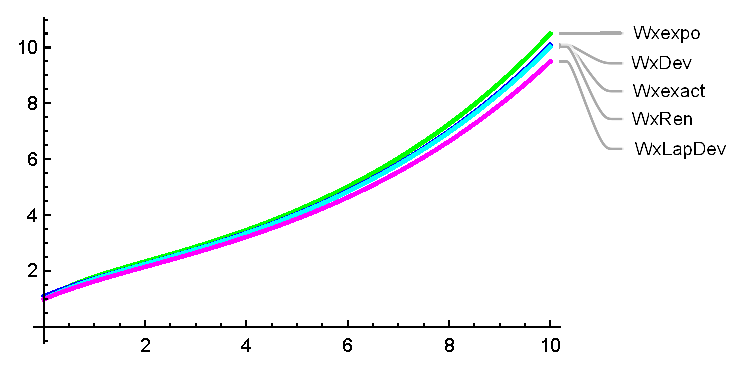
\includegraphics[width=\textwidth]{Wsample1}
        \caption{$W_q(x)$}
        \label{fig:Wsample1}
    \end{subfigure}
    ~ %add desired spacing between images, e. g. ~, \quad, \qquad, \hfill etc. 
      %(or a blank line to force the subfigure onto a new line)
    \begin{subfigure}[b]{0.4\textwidth}
        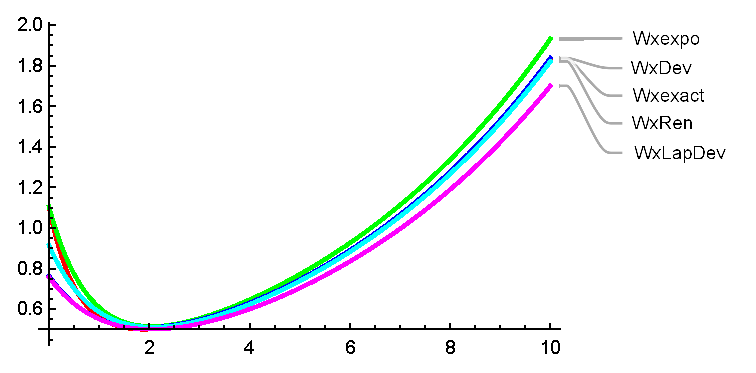
\includegraphics[width=\textwidth]{W1sample1}
        \caption{$W'_q(x)$}
        \label{fig:W1sample1}
    \end{subfigure}
    ~ %add desired spacing between images, e. g. ~, \quad, \qquad, \hfill etc. 
    %(or a blank line to force the subfigure onto a new line)
    \\
    \begin{subfigure}[b]{0.9\textwidth}
        \includegraphics[width=\textwidth]{W2sample1}
        \caption{$W''_q(x)$}
        \label{fig:W2sample1}
    \end{subfigure}
    \caption{Example 1: Plots of $W_q(x)$, $W'_q(x)$, and $W''_q(x)$ of the exact solution and the approximations}\label{fig:sample1}
\end{figure}



\iffalse

The approximation for the \rp\ was already given in Figure \ref{f:MEp1}. The dominant exponents of Renyi and de Vylder are $0.174908, 0.175181$, very close, but a bit smaller than the real $\Fq=0.18198$.

\figu{Wa}{The  Renyi approximation and classic  DeVylder are practically indistinguishable for large $x$
of the exact formula of $W_q(x)$, for $f(x)=\frac{12}{83 }e^{-x}+\frac{42}{83} e^{-2 x}+\frac{150}{83}e^{-3x}$. The   DeVylder-Laplace is rather poor, and so is the naive approximation; overfitting at $0$ seems a bad idea.}{.3}

In  figure \ref{f:Wa}, we draw the exact \sf\ $W_q(x)$, together with the \deV-type and
Renyi    approximations. The figure suggests that the  \re{Renyi \app\ is a lower bound, and that the classic de-Vylder approximation is  the best}. This is investigated in further examples the next section.

As seen in  figure \ref{f:?}   the exact optimal barrier is $b^*=0.866289$, and the Renyi and \re{classic de-Vylder} optimal barriers are \re{$b_R= 0.656067$, ...} 
\fi

\eeXa


\beXa \la{NH5}
Consider the Cram\'{e}r-Lundberg process with density of claims $f(x)=\frac{5}{2 }e^{-5x}+\frac{4}{5} e^{-4 x}-\frac{1}{5}e^{-3x}- \frac{1}{5}e^{-2x}+ \frac{1}{20}e^{-x}$
and $c=\frac{23}{90}$,   $q=\frac{1}{10}$.

One can solve for the other parameters of the process yielding $\l=\frac{7}{12}$, $\th= 1$, $p=23/180$, $\rho = \frac{1}{2}$. The Laplace exponent of this process is $ \kappa(s) = \frac{23 s}{90} -\frac{s}{20 (s+1)}+\frac{s}{10 (s+2)}+\frac{s}{15 (s+3)}-\frac{s}{5 (s+4)}-\frac{s}{2 (s+5)}$ and from here the scale function is
\bea
W_q(x) & = -0.0831561\  e^{(-4.35135 x)} + 0.684818\  e^{(-2.65126 x)} - 0.595164\ e^{(-0.837877 x)} + 6.02604\  e^{(0.666084 x)} \\ & - 2.11949\  e^{(-2.57585 x)} \cos[0.811233 x]  + 2.39748 \  e^{(-2.57585 x)} \sin[0.811233 x]
\eea

\begin{table}[]
\begin{tabular}{|l|l|l|l|l|}
\hline
       & \begin{tabular}[c]{@{}l@{}}Dominant   exponent \\ Phi\_q\end{tabular} & \begin{tabular}[c]{@{}l@{}}Percent   relative error\\ (Phi\_q)\end{tabular} & \begin{tabular}[c]{@{}l@{}}Optimal barrier\\ b*\end{tabular} & \begin{tabular}[c]{@{}l@{}}Percent   relative error\\ (b*)\end{tabular} \\ \hline
Exact  & 0.666084                                                              & 0                                                                           & 0.538                                                        & 0                                                                       \\ \hline
Expo   & 0.691616                                                              & 3.833150173                                                                 & 0.506947                                                     & 5.771933086                                                             \\ \hline
Dev    & 0.670061                                                              & 0.597071841                                                                 & 0.834488                                                     & 55.10929368                                                             \\ \hline
Renyi  & 0.650448                                                              & 2.347451673                                                                 & 0.260532                                                     & 51.5739777                                                              \\ \hline
LapDev & 0.587976                                                              & 11.72644892                                                                 & 0.655954                                                     & 21.92453532                                                             \\ \hline
\end{tabular}
\caption{Example 2: Values of $\Phi_q$ and $b^*$ obtained from the approximations and percent relative error when compared to the exact value}
\label{table:sample2}
\end{table}

\begin{figure}
    \centering
    \begin{subfigure}[b]{0.4\textwidth}
        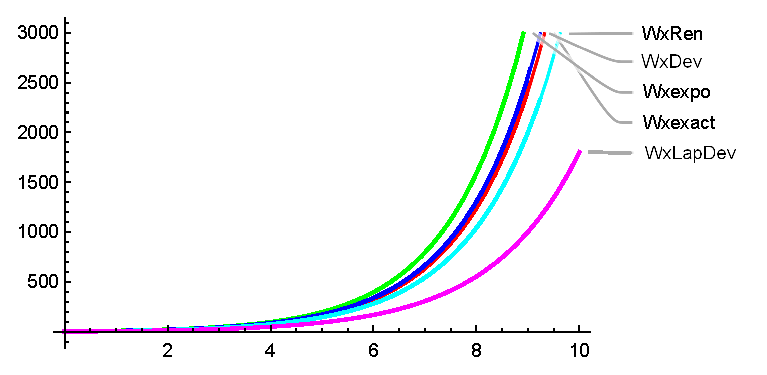
\includegraphics[width=\textwidth]{Wsample2}
        \caption{$W_q(x)$}
        \label{fig:Wsample2}
    \end{subfigure}
    ~ %add desired spacing between images, e. g. ~, \quad, \qquad, \hfill etc. 
      %(or a blank line to force the subfigure onto a new line)
    \begin{subfigure}[b]{0.4\textwidth}
        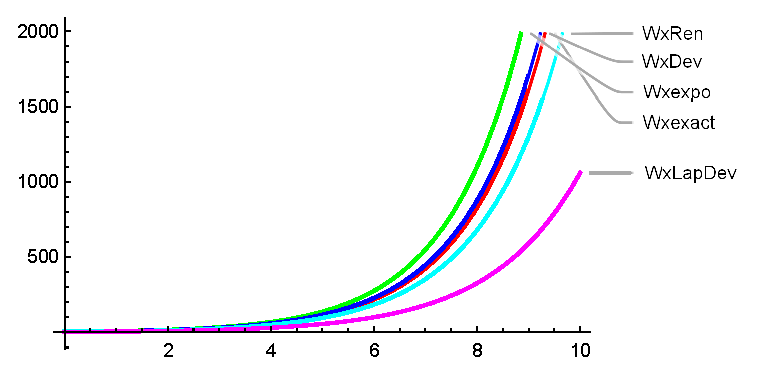
\includegraphics[width=\textwidth]{W1sample2}
        \caption{$W'_q(x)$}
        \label{fig:W1sample2}
    \end{subfigure}
    ~ %add desired spacing between images, e. g. ~, \quad, \qquad, \hfill etc. 
    %(or a blank line to force the subfigure onto a new line)
    \\
    \begin{subfigure}[b]{0.9\textwidth}
        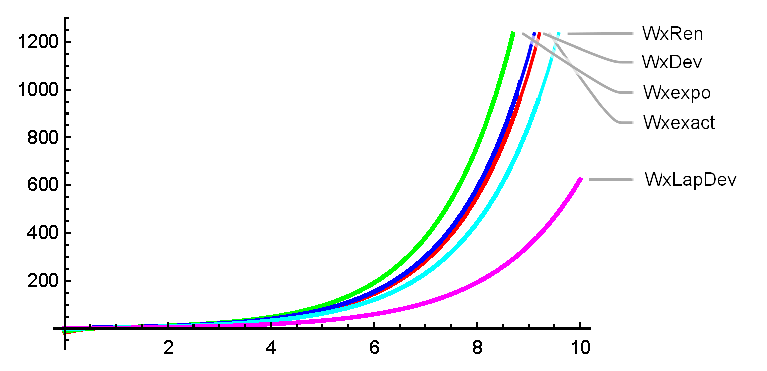
\includegraphics[width=\textwidth]{W2sample2}
        \caption{$W''_q(x)$}
        \label{fig:W2sample2}
    \end{subfigure}
    \caption{Example 2: Plots of $W_q(x)$, $W'_q(x)$, and $W''_q(x)$ of the exact solution and the approximations}\label{fig:sample2}
\end{figure}

The approximations for  $W_q(x)$ give again  Renyi and classic \deV as champions.
The dominant exponents of the Renyi and \deV s are $0.650448$, $0.670061$, one below and one above    the real $\Fq=0.666084$. This suggests that the average of the two approximations would improve on both of them.

\iffalse
\figu{W2}{}{}
\fi


    The exact optimal barrier is $b^*=0.538,$ the Renyi optimal barrier is $b_R= 0.260532$, and the relative error is $0.515739$.
    Both $W_q''$ and its \app\ are increasing \funs.

    --see \cite{johnson1989matching} for more hardest types of approximations; therein the case of mixture of Erlang distributions of sufficiently high common order was investigated.



\eeXa



\beXa

In The following example, we take a Cram\'{e}r-Lundberg process with
\bea c=\frac{7}{18},  \l=\frac{47}{60}, \th= 1\eea
and non-hyperexponential density of claims $f(x)=\frac{5}{2 }e^{-5x}+\frac{4}{5} e^{-4 x}+\frac{1}{5}e^{-3x}- \frac{1}{5}e^{-2x}+ \frac{1}{20}e^{-x}$.

The   scale function is %for the process  in Example \ref{ex1} is
  \bea
  \begin{aligned}
&  W_\q(x)  =  -0.083013\ 2.71828^{(-4.45457 x)} - 0.193651\ 2.71828^{(-3.43626 x)} -
 0.459603\ 2.71828^{(-0.855781 x)} \\
  & + 4.15668\ 2.71828^{(0.454369 x)} -  0.84898\ 2.71828^{(-2.21816 x)} \cos[0.513884 x] + 1.24626\ 2.71828^{(-2.21816 x)} \sin[0.513884 x]
\end{aligned}
  \eea

\begin{table}[]
\begin{tabular}{|l|l|l|l|l|}
\hline
       & \begin{tabular}[c]{@{}l@{}}Dominant   exponent \\ Phi\_q\end{tabular} & \begin{tabular}[c]{@{}l@{}}Percent   relative error\\ (Phi\_q)\end{tabular} & \begin{tabular}[c]{@{}l@{}}Optimal barrier\\ b*\end{tabular} & \begin{tabular}[c]{@{}l@{}}Percent   relative error\\ (b*)\end{tabular} \\ \hline
Exact  & 0.420145                                                              & 0                                                                           & 0.797999                                                     & 0                                                                       \\ \hline
Expo   & 0.429586                                                              & 2.247081365                                                                 & 0.857445                                                     & 7.449382769                                                             \\ \hline
Dev    & 0.420885                                                              & 0.17612967                                                                  & 0.0686674                                                    & 91.39505187                                                             \\ \hline
Renyi  & 0.416601                                                              & 0.843518309                                                                 & 0.794273                                                     & 0.466917878                                                             \\ \hline
LapDev & 0.392412                                                              & 6.600816385                                                                 & 0.271363                                                     & 65.99456892                                                             \\ \hline
\end{tabular}
\caption{Example 3: Values of $\Phi_q$ and $b^*$ obtained from the approximations and percent relative error when compared to the exact value}
\label{table:sample3}
\end{table}


\begin{figure}
    \centering
    \begin{subfigure}[b]{0.4\textwidth}
        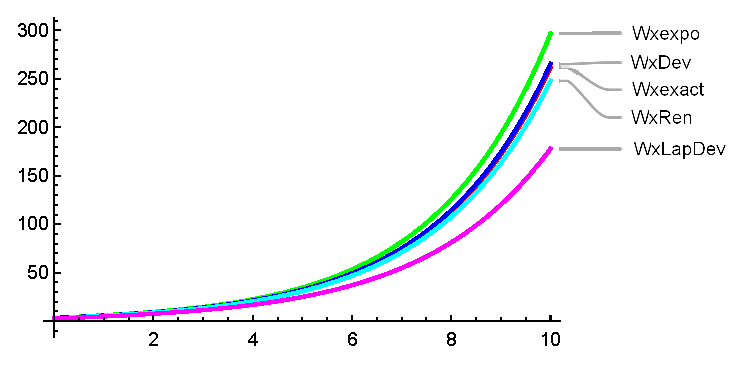
\includegraphics[width=\textwidth]{Wsample3}
        \caption{$W_q(x)$}
        \label{fig:Wsample3}
    \end{subfigure}
    ~ %add desired spacing between images, e. g. ~, \quad, \qquad, \hfill etc. 
      %(or a blank line to force the subfigure onto a new line)
    \begin{subfigure}[b]{0.4\textwidth}
        \includegraphics[width=\textwidth]{W1sample3}
        \caption{$W'_q(x)$}
        \label{fig:W1sample3}
    \end{subfigure}
    ~ %add desired spacing between images, e. g. ~, \quad, \qquad, \hfill etc. 
    %(or a blank line to force the subfigure onto a new line)
    \\
    \begin{subfigure}[b]{0.9\textwidth}
        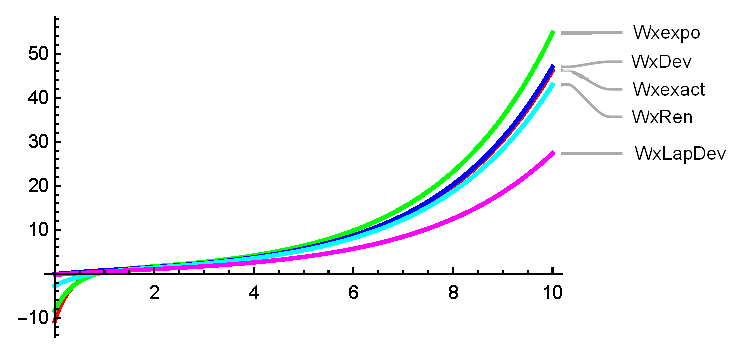
\includegraphics[width=\textwidth]{W2sample3}
        \caption{$W''_q(x)$}
        \label{fig:W2sample3}
    \end{subfigure}
    \caption{Example 3: Plots of $W_q(x)$, $W'_q(x)$, and $W''_q(x)$ of the exact solution and the approximations}\label{fig:sample1}
\end{figure}

In this case, the approximations for  $W_q(x)$ give Renyi as winner.
The dominant exponents of the Renyi and \deV s are $0.44982$, $0.455485$, one below and one above    the real $\Fq=0.454369$.
\iffalse
\figu{Wa2a}{}{}
\fi

    The exact optimal barrier is $b^*=0.779653,$ the Renyi optimal barrier is $b_R=0.732339$, and the relative error is $0.060686$.
    Both $W_q''$ and its \app\ are increasing \funs.


\eeXa



\beXa
Next we consider a more challenging example from BUTools,   produced by taking
a Cram\'{e}r-Lundberg process with matrix exponential, non phase-type  density of claims $f(x)=\a e^{A x} (-A) \bff 1, $ where $\a=(-2.4, 0.9 , 2.5),  A = \bep
   {-6.2, 2, 0}\\
   {2, -9, 1}\\
   {1, 0, -3}\eep$
and $  \th= 1, q=1/10.$

--see \cite{harris1992note} and \cite{reintelek14} for other tricky densities.


The   scale function is %for the process  in Example \ref{ex1} is
  \bea
  \begin{aligned}
& -0.0655864 e^{-9.35143 x}+0.149742 e^{-6.89805 x}-0.676982 e^{-1.26245 x}+1.3476 e^{0.142175 x}
\end{aligned}
  \eea

\iffalse
\figu{Wa3a}{}{}
\fi

 Now $\Fq=0.142175$; the dominant exponent of the classic \deV\ is very close at $ 0.142174$, and the dominant exponent of Renyi, $0.142238$, is also close.




    The exact optimal barrier is $b^*=2.61925$,   the Renyi optimal barrier is $b^*= 2.59638$, and the relative error is $0.00873044$. For classic \deV\,
    the relative error is $0.00609153$.

    However,  we may have a surprise in  examples where $b^*$ is not the unique root of $W_q''(x)$, and we may be faced with the Azcue-Muller-Loeffen phenomenon.

\iffalse    
    \figu{pl3}{When $W_q''(x)$  exhibits oscillations, exponential approximations are bound to fail in certain regions. In our example, the minimum of $W'_q$ is still unique; otherwise, one may need to resort to higher order  Pad\'e and  Laguerre  approximations. Producing examples where $W_q''(x)$   exhibits more than   three roots
and investigating the convergence of the roots of our Pad\'e approximations  seem both  hard problems.}{}
\fi
\eeXa

\iffalse
\beXa
Inspired by the density given in \cite{harris1992note}, we take in the following example a \CL \ process with
$$ \th = \frac{48}{55}, \quad \mbox{and}\ \l =1$$
with non-hyperexponential density of claims given by
$ f(x)= 3 e^{-x} - 6 e^{- 2x} +3 e^{- 3x}$
the scale function is :
 \bea \begin{aligned} & W_q (x) = -0.280452\ 2.71828^{(-0.421202 x)} + 0.540968\ 2.71828^{(0.0578629 x)} +
 0.0307461\ 2.71828^{(-2.65814 x)} \cos[0.323643 x] \\
  &+ 0.0791481\ 2.71828^{(-2.65814 x)} \sin[0.323643 x] \end{aligned} \eea

Similar to the previous example of a non-phase-type density, the approximation of $W_q$ give the classic DeVylder approximation as winner.
 \figu{wa4}{}{}

 The exact optimal barrier is  $b^*=6.9158 $,   the Renyi optimal barrier is $b_R= 6.79333$, and the relative error is $9.46103$.
 $\Phi_q = 0.0578629$; The dominant exponents of the Renyi is close at $0.0578967$ and the dominant exponent of the classic DeVylder is very close at $0.0578619.$

\figu{wsec4}{}{}

\eeXa


\beXa
We take advantage of the example presented in \cite{reintelek14}; now by taking
a Cram\'{e}r-Lundberg process with matrix exponential, non phase-type  density of claims $f(x)=\a e^{A x} (-A) \bff 1, $ where $\a=(3.99334, -5.99002, 4.32612, -1.99667, 0.667221),  A = \bep
   {-1, 1, 0, 0, 0}\\
 {0, -1, 1, 0, 0}\\
 {0, 0, -1, 1, 0}\\
 {0, 0, 0, -1, 1}\\
 {0, 0, 0, 0, -1}
\eep$ and $  \th= 1, q=1/10$.
\figu{wPH}{}{}

In this case the classic DeVylder approximation is the champion.

\figu{wPH2}{}{}

Now $\Phi_q = 0.016699$;  the dominant exponent of the classic \deV\ is very close at $ 0.0166987$, and the dominant exponent of Renyi, $0.0167116$, is also close.



 The exact optimal barrier is $b^*=21.7388 $,   the Renyi optimal barrier is $b_R= 21.7041$, and the relative error is $0.00159435 $.
\eeXa


\beXa
Another very interesting example, also inspired from \cite{reintelek14}, but this time
we take a Cram\'{e}r-Lundberg process with matrix exponential, non phase-type  density of claims $f(x)=\a e^{A x} (-A) \bff 1, $ where $\a=(1, -0.7, 0.7),  A = \bep
 {-2, 2, 0}\\
 {0, -5, 5}\\
 {0, 0, -9}
\eep$ and $  \th= 1, q=1/10$.
\figu{wPH0}{}{}
 Here the classic \deV\ approximation is also the winner.



Now $\Phi_q =0.137583 $;  the dominant exponent of the classic \deV\ is very close at $ 0.137579$, and the dominant exponent of Renyi, $0.137688$, is also close.
\figu{wPH1}{}{}



 The exact optimal barrier is $b^*=2.91429  $,   the Renyi optimal barrier is $b_R= 2.81849 $, and the relative error is $ 0.0328731  $.


 Note that the Exact $W'$ diverge from the plot of the classic Renyi, \figu{wRn}{}{}

 and so as in the plot of the Naive approximation of $W$ and the Exact $W''$. \figu{wNa}{}{}

\eeXa

\beXa
In the following example, for a Cram\'er Lundberg model we take the hyperexpoential density of claims given in \cite{avram2011moments} by  $f(x)= \frac{315}{12 }e^{-5x}+\frac{7}{8} e^{-4 x}+\frac{27}{64}e^{-3x}+ \frac{3}{16}e^{-2x}+ \frac{7}{128}e^{-x}$, with $\th = \frac{48}{55}$;


The scale function is

\bea \begin{aligned}
& W_q (x)= -0.00493814\ 2.71828^{(-4.07091 x)} - 0.0558297\ 2.71828^{(-3.19893 x)} -
 0.196449\ 2.71828^{(-2.54279 x)}\\
 & - 0.123323\ 2.71828^{(-1.83918 x) }- 0.0646808\ 2.71828^{(-0.941267 x)} + 0.87134\ 2.71828^{(0.0892008 x)} \end{aligned}\eea
\figu{wAv}{}{}

We notice again that the classic DeVylder is the winner.


And here $\Phi_q = 0.0892008$; the dominant exponent of the classic \deV\ is very close at $ 0.0892021$, and the dominant exponent of Renyi, $0.0891807$, is also close.
\figu{wAv0}{}{}


The exact optimal barrier is $b^*=2.70201 $,   the Renyi optimal barrier is $b_R= 2.74935 $, and the relative error is $0.0175198  $.


\eeXa

\fi

    \iffalse


    {\bf The Pad\'e Tijms \app \ is $b^*=0.876898$}.
    %
The input to the \LTW \ inversion is
     \[ \H G (s)=\frac{216 \left(261 s^2+1155 s+1202\right)}{187 (6 s+5) (6 s+11) (6 s+17)},\]
the  Pad\'e approximation of order $(0,1)$ is $\frac{312077664}{187 (1278399 s+1123870)}$,  the Laguerre exponent is $\alpha/2=0.879123$, and the largest error with $n=40$ is $4 \times 10^{-14}$ -- see Figure \ref{f:err3}.
\figu{err3}{Relative errors of the \LTW \ inversion with mixed exponential claims of order $3$}{}

Again, the exponent  $\alpha/2=\fr{ 6 \k'(\Fq) \k''(\Fq)}{3 (\k''(\Fq))^2- \k'(\Fq) \k'''(\Fq)}=1.138$ does better,  with the largest error  with $n=40$ of $6 \times 10^{-16}$.  This suggests the importance of optimizing $\a$, which is a  difficult problem \cite{giunta1989more,weideman1999algorithms}.  Recall however our proposal  to circumvent it by starting with a
higher order \Pd \ of $G(s)$ -- see \eqref{MG}.
 Another reasonable choice is the ``true dominant exponent  $\alpha/2=5/6$ which is unknown in real life, and yields a larger error $3 \times  10^{-15}$ (with $n=50$). The exponent of the new  formula \eqref{al} is $\alpha/2=0.77$, and the  error with $n=50$ is $3 \times 10^{-14}$, even larger.
%\fi
In  the figure \ref{f:MEp2}, we draw the exact $W_q$, together with its six   approximations.
\fi
\iffalse


 \figu{}{\label{Erl(2)} Approximations of the scale function pour sinistres Erlang(2,2), $\r=.84$ en gras pointill\'e, avec Tijms tr\`es proche dessous. L'approx. exponentielle en bas est la pire. De Vylder (pointill\'e) et Renyi sont tr\`es proches pour $u>3$, et leur moyenne fait encore mieux pour $u<3$.}
{0.7}
\fi


%\input{two}

\small
\bibliographystyle{amsalpha}
%\bibliographystyle{plain}
\bibliography{Pare37}

\end{document}



